\documentclass[Space_Shuttle_Vessel_Manual.tex]{subfiles} 
\begin{document}

\section{SSV and Orbiter Space Flight Simulator}
\begin{multicols*}{2}
\renewcommand{\cfttoctitlefont}{\bf}
\localtableofcontents
\noindent
\\
The section provides information about how to operate Space Shuttle Vessel in Orbiter Space Flight Simulator.

%Orbiter Vehicle, its configuration and coordinate system, the nominal mission profile, and general procedures followed during a shuttle mission.
%Also included in this section is keyboard commands for SSV but will not include standard Orbiter Simulator keyboard commands. See Orbiter.pdf for standard Orbiter Simulator keyboard commands.
\end{multicols*}


\newpage
\subsection{SSV Keyboard Commands}
\begin{multicols*}{2}
The ultimate goal of SSV is to provide a complete simulation of the Space Shuttle.  This means that most of the input is done with in-simulation controls (i.e. cockpit switches, GPC keyboards, and dialog windows). This results in very few keyboard commands to operate the shuttle.\\

\textbf{General}\\
Ctrl+A - toggle between CDR/PLT/AFD RHC and THC, and RMS RHC and THC\\
Ctrl+G - arm landing gear\\
G - deploy landing gear\\
\vspace{\baselineskip}

\textbf{RMS}\\
Ctrl+Enter - grapple\\
Ctrl+Backspace - release\\
Ctrl+O - toggle between Coarse and Vernier rates\\

\subsection{Rotational Hand Controller / Translational Hand Controller}
The regular Orbiter Space Flight Simulator thruster control commands (either keyboard or joystick) are used to simulate the Rotational Hand Controller (RHC) \& Translational Hand Controller (THC). To use the RHC and THC, the associated \textit{FLT CNTLR PWR} switch must be on, as well as the associated (Display Driver Unit) DDU. For the RMS RHC and THC, the RMS needs to be powered.
\\
\\
The RHCs on the real shuttle have a "soft stop" and a "hard stop" (the mechanical limit of movement). Moving the RHC out of detent (up to the soft stop) will command either a constant rotation rate or a pulse of RCS firings to change the rotation rate by a specified amount (depending on whether \textit{DISC RATE} or \textit{PULSE} has been selected). Moving the RHC past the soft stop will result in continuous thruster firings in the appropriate axis. In SSV, a thruster command of <75\% is considered to be within the soft stop; a thruster command of >75\% is treated as RHC deflection beyond the soft stop. When using keyboard controls, the normal keyboard controls are equivalent to full RHC deflection, while holding down the Ctrl key is equivalent to deflection within the soft stop. The THC (and the RMS controls) does not have this idea of a soft stop. When \textit{NORM} is selected in a translational axis, the thrusters will fire continuously if the THC is moved out of detent. When \textit{PULSE} is selected, the thrusters will fire to provide a specified $\Delta$V (the TRAN PLS rate specified on the SPEC 20 DAP CONFIG display). When controlling the RMS, the commanded rotation/translation rates are always directly proportional to the RHC/THC deflection.\\
RHC trim switches are commanded with the Shift+Arrow Key.

\begin{figure}[H]
  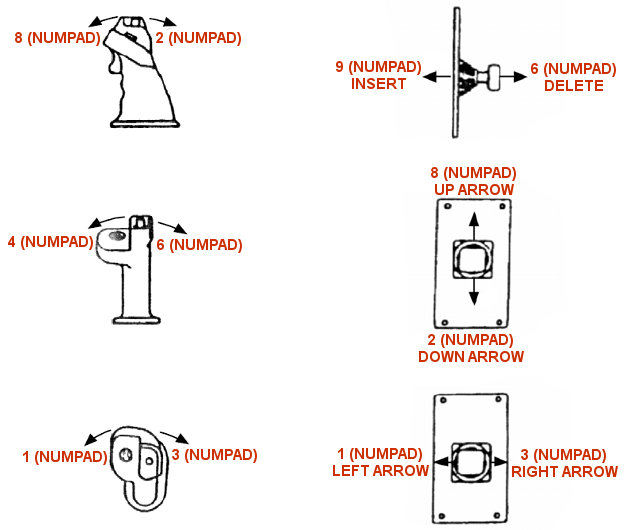
\includegraphics[width=0.99\hsize]{RHC_THC_keys.png}
  \caption{RHC/THC key mapping}
  \label{fig:RHC_THC_keys}
\end{figure}

\subsection{Speedbrake/Thrust Controller}
The Speedbrake/Thrust Controller (SBTC) controls both SSME throttling during ascent and the speedbrake setting during entry. In Orbiter, the SBTC is controlled in 5\% intervals, in the forward direction by the numpad \textit{Subtract} key, and in the aft direction via the numpad \textit{Add} key. The takeover switch, used to initiate manual control of the SSME throttle or speedbrake settings, is simulated by the \textit{Minus} key. The appropriate \textit{FLT CNTLR PWR} switch must be on, as well as the appropriate DDU, for the SBTC to be active. Each SBTC is animated so the user can tell what setting is being commanded. During ascent, a full aft SBTC position corresponds to MPL (Minimum Power Level), usually 65 or 67\% SSME throttle; full forward SBTC position corresponds to the current maximum SSME throttle, a value ranging from 100 to 109\%, depending on mission or abort case. During landing, full aft SBTC position corresponds to the speedbrake being \textbf{fully open}; full forward SBTC position corresponds to the speedbrake being commanded \textbf{fully closed}.

\paragraph{Ascent}
During ascent, SSME throttling is usually controlled by autopilot; in this case, the \textit{AUTO} portion of the \textit{SPD BK/THROT} PBIs on Panel F2 \& Panel F4 is lit, and \textbf{THRTL: Auto} is displayed in the A/E PFD display. To takeover manual control of the SSME throttle command, press the SBTC takeover switch and move the SBTC to match the current SSME auto command (displayed in the Ascent Traj displays). When the SBTC takeover switch is pressed both \textit{AUTO} PBIs will go out, indicating a manual takeover is in progress, but not completed. When the SBTC-commanded SSME throttle setting matches the auto command within 4\%, the PLT \textit{SPD BK/THROT MAN} PBI will be lit and \textbf{THRTL: Man} appears in the A/E PFD display, indicating that the SSME throttle is now under manual control. To return to auto SSME throttle control, press either \textit{SPD BK/THROT MAN} PBI. A manual MECO can be commanded by pressing the NUMPAD * key (in real life, this is done by simultaneously pressing all 3 \textit{MAIN ENGINE SHUT DOWN} push buttons on Panel C3; this is not possible in Orbiter).

\paragraph{Entry}
\label{sec:entry}
The speedbrake is usually controlled automatically throughout entry, with the \textit{AUTO} portion of the \textit{SPD BK/THROT} PBIs on Panel F2 \& Panel F4 is lit, and \textbf{SB: Auto} is displayed in the A/E PFD display. To take over manual control of the speedbrake press the SBTC takeover switch; the speedbrake will immediately move to the position commanded by the SBTC, the \textit{AUTO} portion of the \textit{SPD BK/THROT} PBIs will go out and the \textit{MAN} PBI will be lit on either the CDR or PLT position (depending on what SBTC takeover switch was last pressed). Pressing the either \textit{SPD BK/THROT} PBI, will put the speedbrake into \textit{AUTO} mode again.

\subsubsection{Rudder Pedal Transducer Assembly}
The Rudder Pedal Transducer Assembly (RPTA) allows manual control of the rudder during the later part of reentry, as well as the Nose Wheel Steering during rollout. The RPTA also contains the brake pedals, which in addition to braking provide another means of lateral control during rollout. Although the rudder is automatically controlled, manual control is available when the R/Y channel is in CSS. The appropriate \textit{FLT CNTLR PWR} switch must be on, as well as the appropriate DDU, for the RPTA to be active.




\begin{figure}[H]
  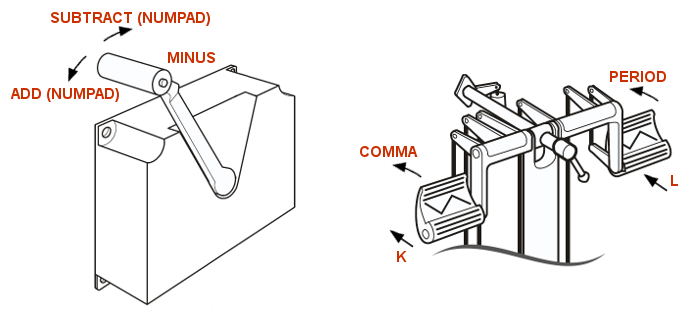
\includegraphics[width=0.99\hsize]{SBTC_RPTA_keys.png}
  \caption{SBTC/RPTA key mapping}
  \label{fig:SBTC_RPTA_keys}
\end{figure}


\subsection{Camera Views}
SSV includes the four payload bay cameras, the 2 RMS cameras and the Orbiter Docking System (ODS) centerline camera. The PLB and Elbow RMS cameras are controlled from panel A7U on the flight deck. In the PLB and RMS camera VC views, the cameras can also be controlled using Alt+Arrow keys.

\subsection{Navigating the Virtual Cockpit}
SSV has several Virtual Cockpit (VC) positions, allowing the user to navigate between the main locations and station of the crew module. Table \ref{tab:VC_navigation} lists all the available VC positions, as well as neighbour positions accessed with the standard Ctrl+Arrow key combination. Each position also has lean positions (Alt Gr+Arrow key) which allow better positioning to reach a specific panel or window.\\
For assistance in navigating the VC, the name of the position is shown for a few seconds at the top of the screen during the simulation.
\\

\end{multicols*}
\begin{table}[H]
\begin{threeparttable}
  \centering
  \begin{tabular}{l|p{2.88cm} p{2.88cm} p{2.88cm} p{2.88cm} }
	\textbf{Cockpit View} & \textbf{Left} & \textbf{Right} & \textbf{Up} & \textbf{Down} \\
	\hline\rule{0pt}{2ex}
	Commander Seat & CDR - L4 & Pilot Seat & PLB Camera A \textit{or} ODS Camera\tnote{c} & MS Seat \\
	\hline\rule{0pt}{2ex}
	Pilot Seat & Commander Seat & Pilot - R4 & PLB Camera D \textit{or} ODS Camera\tnote{c} & MS2/FE Seat \\
	\hline\rule{0pt}{2ex}
	CDR - L4 & Port Workstation & Commander Seat & PLB Camera D \textit{or} ODS Camera\tnote{c} & MS Seat \\
	\hline\rule{0pt}{2ex}
	Pilot - R4 & Pilot Seat & Stbd Work Station & PLB Camera D \textit{or} ODS Camera\tnote{c} & MS2/FE Seat \\
	\hline\rule{0pt}{2ex}
	MS Seat & Port Workstation & MS2/FE Seat & Commander Seat & PLB Camera A \textit{or} ODS Camera\tnote{c}\\
	\hline\rule{0pt}{2ex}
	MS2/FE Seat & MS Seat & Stbd Work Station & Pilot Seat & PLB Camera A \textit{or} ODS Camera\tnote{c}\\
	\hline\rule{0pt}{2ex}
	Port Work Station & RMS Work Station & Commander Seat & PLB Camera A \textit{or} ODS Camera\tnote{c} & Mid Deck\\
	\hline\rule{0pt}{2ex}
	Stbd Work Station & Pilot Seat & Aft Pilot Station & PLB Camera D \textit{or} ODS Camera\tnote{c} & Aft Work Station\\
	\hline\rule{0pt}{2ex}
	Aft Work Station & Stbd Work Station & Port Workstation & RMS Work Station & MS Seat\\
	\hline\rule{0pt}{2ex}
	Aft Pilot Station & Stbd Work Station & RMS Work Station & PLB Camera D \textit{or} ODS Camera\tnote{c} & Aft Work Station\\
	\hline\rule{0pt}{2ex}
	RMS Work Station & Aft Pilot Station & Port Work Station & PLB Camera A \textit{or} ODS Camera\tnote{c} & Aft Work Station\\
	\hline\rule{0pt}{2ex}
	RMS EE\tnote{a} & RMS Elbow & - & - & RMS Work Station\\
	\hline\rule{0pt}{2ex}
	RMS Elbow\tnote{a} & - & RMS EE & - & RMS Work Station\\
	\hline\rule{0pt}{2ex}
	PLB Camera A & PLB Camera D & PLB Camera B & RMS EE\tnote{a,c} & RMS Work Station \textit{or} ODS Camera\tnote{c}\\
	\hline\rule{0pt}{2ex}
	PLB Camera B & PLB Camera A & PLB Camera C & RMS EE\tnote{a,c} & RMS Work Station \textit{or} ODS Camera\tnote{c}\\
	\hline\rule{0pt}{2ex}
	PLB Camera C & PLB Camera B & PLB Camera D & RMS EE\tnote{a,c} & Aft Pilot Station \textit{or} ODS Camera\tnote{c}\\
	\hline\rule{0pt}{2ex}
	PLB Camera D & PLB Camera C & PLB Camera A & RMS EE\tnote{a,c} & Aft Pilot Station \textit{or} ODS Camera\tnote{c}\\
	\hline\rule{0pt}{2ex}
	ODS Camera\tnote{c} & - & - & PLB Camera A & Aft Pilot Station\\
	\hline\rule{0pt}{2ex}
	Mid Deck & - & - & Port Work Station & External Airlock\tnote{b}\\
	\hline\rule{0pt}{2ex}
	External Airlock\tnote{b} & - & - & Mid Deck & ODS Camera\tnote{c}\\
  \end{tabular}
	\begin{tablenotes}
		\item[a] only when RMS is installed
		\item[b] only when External Airlock is installed
		\item[c] only when ODS is installed
	\end{tablenotes}
	\end{threeparttable}
  \caption{VC navigation}
  \label{tab:VC_navigation}
\end{table}


\begin{multicols*}{2}
\subsection{Atmospheric Wind}
In addition to planetary surface elevation, the 2016 version of Orbiter Space Flight Simulator also implements atmospheric winds.\\
Unlike the real world, there is no weather forecast in Orbiter, so during landing it is easy to fly the vehicle into a wind situation that exceeds its (narrow) operating capabilities. For this reason, if atmospheric wind effects are enabled, intense monitoring of the vehicle performance during landing is required to ensure the vehicle reaches the runway.\\


\subsection{Options}
The file <Orbiter installation>\textbackslash Config\textbackslash Vessels\textbackslash SSV\_OV.cfg file contains parameters to control some features of the Orbiter Vehicle vessel.\\
Table \ref{tab:OptionParameterList} lists all the available option parameters.

\end{multicols*}

\begin{table}[H]
  \centering
  \begin{tabularx}{470pt}{c | >{\centering\arraybackslash}p{50pt} | >{\centering\arraybackslash}p{300pt}}
    \textbf{Parameter} & \textbf{Type} & \textbf{Description} \\
    \hline
	EIUDataRecorder & bool & Enables output of SSME controller data to file <Orbiter installation>\textbackslash EIU\_data\_ch<id>.txt\\
	\hline\rule{0pt}{2ex}
	PositionLabelTime & integer & Controls duration of vc position label output, [0;60] seconds\\
	\hline\rule{0pt}{2ex}
	AutoActionLandingGear & bool & Enables automatic Landing Gear arm and deploy\\
	\hline\rule{0pt}{2ex}
	AutoActionDragChute & bool & Enables automatic Drag Chute deploy and jettison
	\end{tabularx}
  \caption{Option Parameter List}
  \label{tab:OptionParameterList}
\end{table}

\end{document}